\section{Methods}

\begin{figure*}[t]
\centering
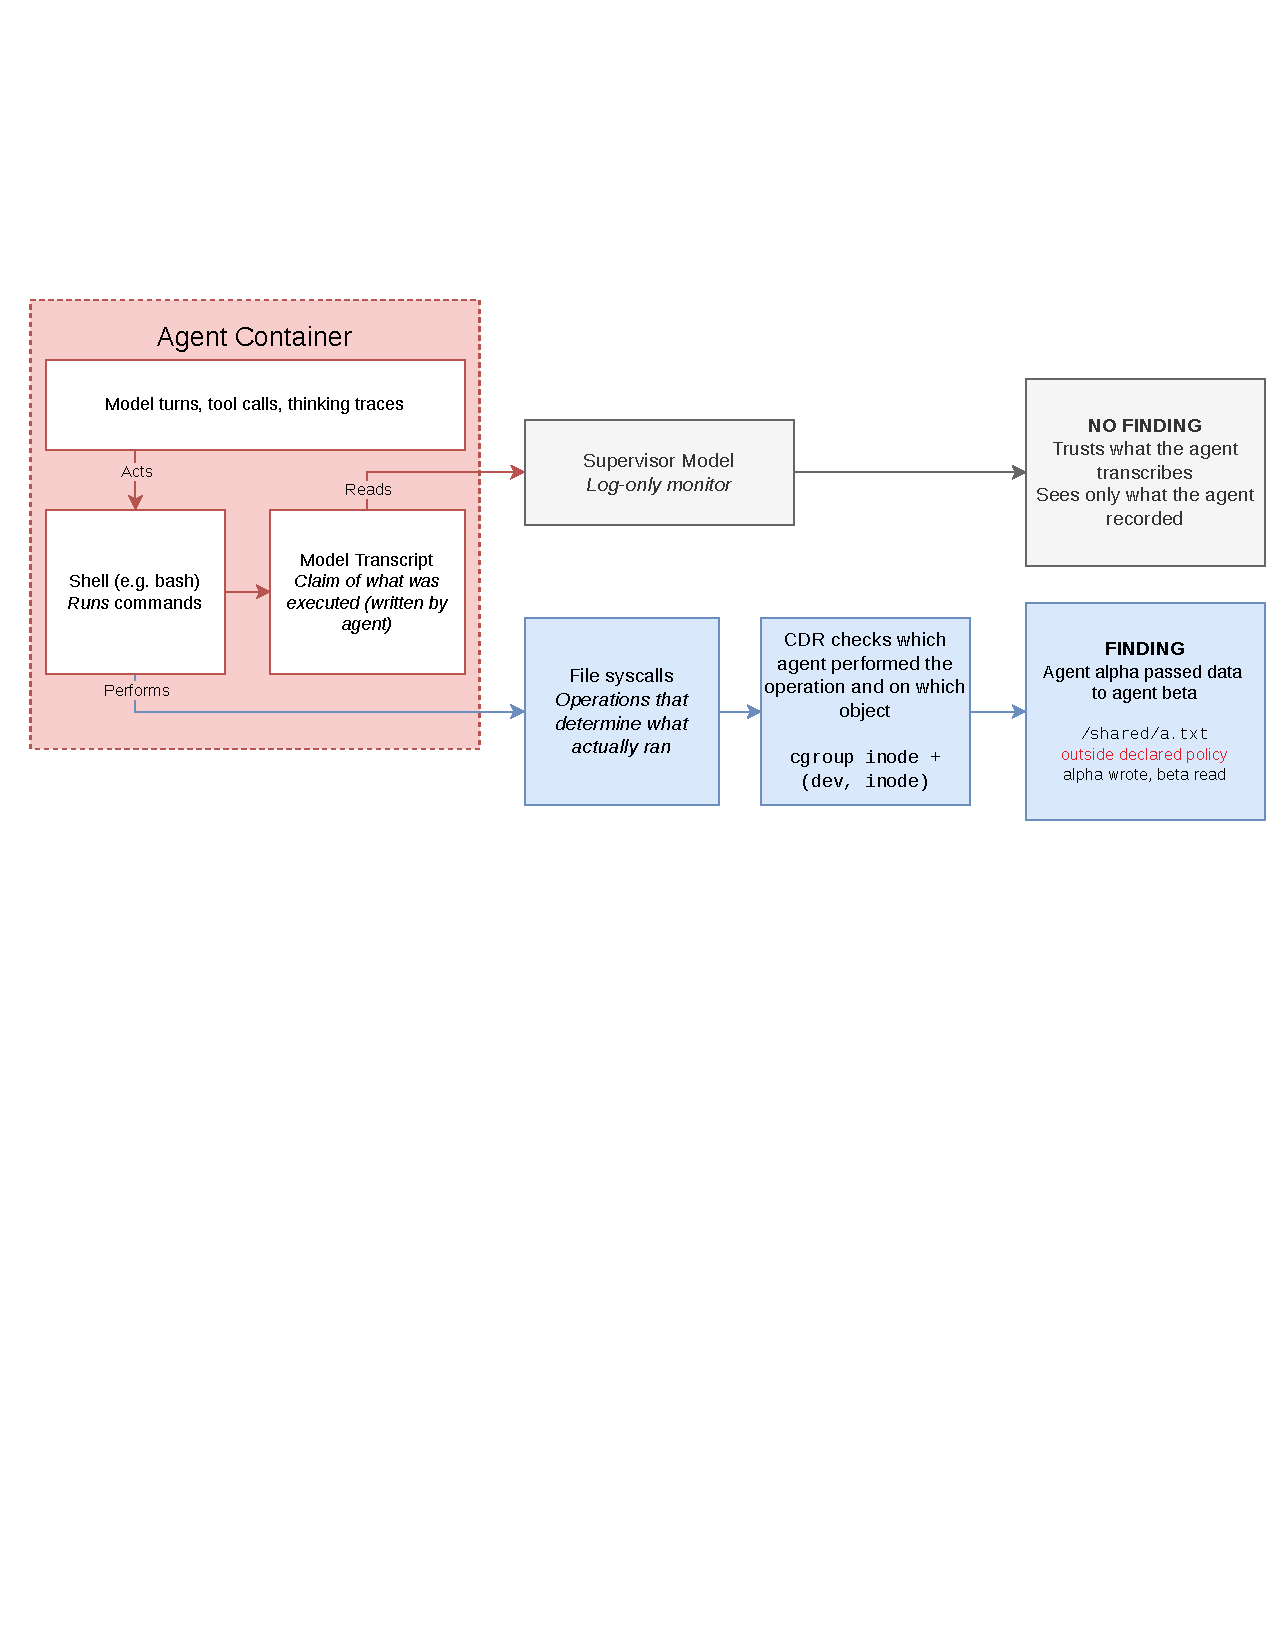
\includegraphics[width=\textwidth]{figures/fig1.pdf}
\caption{Inside the dashed container, everything is written by the agent and can be rewritten by it, so the transcript is a claim. The supervisor model has no input but that claim, and cannot separate a forged transcript from an honest one that simply omits the action. The kernel witnesses the syscall instead, resolves which agent performed the operation and on which object, and emits the edge when two agents touch the same object. The object is joined on device and inode, and the path is shown only for the reader. Agents \texttt{alpha} and \texttt{beta} are two containers in a sandbox slice.}
\label{fig:trust}
\end{figure*}

Figure~\ref{fig:trust} summarises the arrangement the rest of this section builds. Everything inside the dashed container is controlled by the agent and can be modified by it, whereas everything outside is recorded by the kernel. The mechanism exists so that a verdict depends only on the right-hand side, and every design choice below is an attempt to move a piece of substantiated evidence across that boundary.

\noindent\textbf{Identity.} No field of an agent's identity is left self-reported. A cgroup is the kernel's own grouping of processes, fixed when the process is created and exposed as a directory tree. An agent is the cgroup v2 inode it belongs to, read via \texttt{bpf\_get\_current\_cgroup\_id()} at syscall entry and resolved to the nearest registered ancestor in the sandbox subtree. A container-per-agent deployment needs no further configuration for CDR to function. Where several agents share a single container, however, the harness must create child cgroups and declare them to the loader out of band so that the agents become separable. We first accepted any nested cgroup whose name matched a designated prefix, and we rejected it after reviewing the security implications: an agent with the capability to create cgroups could adopt a neighbour's name, or create several identities and split its own behaviour across them, which manufactures edges between two halves of one attacker. A name the subject chooses cannot be an identity, so declarations are supplied by the deployment and nested cgroups that were not declared resolve to their nearest declared ancestor. An agent therefore cannot acquire an identity by creating a directory.

\noindent\textbf{Objects.} Objects are joined on what the kernel knows, not on what the agent called them. Events are keyed on the pair $(\mathit{device},\mathit{inode})$ rather than on the inode alone, because inode numbers repeat across containers that share image layers. In our testbed, the shared volume collapses to a single key, $29/2693466$, for every agent, while the same binary in three containers appears as inode $2604173$ under devices $85$, $74$ and $82$. Keying on the inode alone would report every agent that launches \texttt{bash} as sharing an object with every other, whereas keying on the pair separates them without any knowledge of file names.

\noindent\textbf{Capture.} The probe does not need to know which channels exist in order to spot them. Ring-0 holds no per-syscall knowledge. For every syscall in the slice, the probe records the syscall number, its arguments, the cgroup, and up to two user strings, chosen by a bitmap the loader derives at startup from the kernel's own tracepoint metadata. An argument is marked when it is typed \texttt{char *} and its name indicates a path. Vectors such as \texttt{execve} arguments are read element-wise onto a separate payload ring so they are not truncated. Adding a syscall is a map insertion instead of a recompilation. Syscalls outside the bitmap are counted per-agent rather than discarded, so an unmodelled channel surfaces as a frequency anomaly against the benign baseline instead of as silence. Local sockets illustrate the generality of this approach: the name of an \texttt{AF\_UNIX} endpoint sits behind a pointer to a structure rather than in a path argument, so the probe reads the 2-byte address family and follows \texttt{sun\_path} only when the family is \texttt{AF\_UNIX}. Channels are not enumerated anywhere in code.

\noindent\textbf{Resolution.} A path means nothing until it is resolved inside the container that wrote it. The loader resolves each one with \texttt{openat2} using \texttt{RESOLVE\_IN\_ROOT} and \texttt{RESOLVE\_NO\_MAGICLINKS} against an \texttt{O\_PATH} descriptor for the agent's \texttt{/proc/<pid>/root}, then \texttt{fstat}s the result. Both flags exist because of observed failures in testing: an absolute symlink target was otherwise resolved against the host's root, and \texttt{..} at the container root escaped to a host inode shared by every container, each producing false edges. Results are cached by $(\mathit{agent},\mathit{path})$ and invalidated on \texttt{O\_CREAT}, since a delete-and-recreate can be served a different inode. Because \texttt{bind} and \texttt{creat} create their object during the call, resolution at entry necessarily fails (the file does not exist yet), so such an event is retried a finite number of times, and a cached root that outlives its process falls back from the open descriptor to the cached prefix and finally to the calling thread's own \texttt{/proc/<tid>/root}.

\noindent\textbf{Attribution.} Every syscall can be traced to the declaration that authorised it, as a containment claim rather than a proof. The \texttt{sched\_process\_fork} tracepoint yields parent and child, and \texttt{execve} yields the argument vector. Together, they form an exec forest for a given agent, where any declared tool call can be bound to the node whose effective command matches it, after unwrapping one shell level and comparing basenames, and that node's subtree is the delegated action. Every object touch carries a thread-group identifier, so that an edge can be walked back to the declaration that authorised it.

\noindent\textbf{Verdicts.} The detector records what agents did; the policy decides whether it was permitted. Declarations are reconciled against executions into four classes: \texttt{match}, \texttt{mismatch} for a declaration with no accompanying execution, \texttt{omission} for silence, and \texttt{surplus} for an execution with no covering declaration. Separately, each edge is evaluated against a sanction set over paths, yielding sanctioned or unsanctioned. Collusion is defined as an unsanctioned edge. Syscalls are classified as mutators or sensors, and a syscall we have not classified defaults to sense, so any novel communication medium participates as an undirected adjacency rather than being dropped.

